\documentclass[11pt,letterpaper,boxed]{hmcpset}
\usepackage{fullpage}
\setlength{\parskip}{6pt}
\setlength{\parindent}{0pt}
\usepackage[margin=1in]{geometry}
\usepackage{graphicx}
\usepackage{enumerate}
\usepackage{marvosym}
\usepackage{amssymb}
\usepackage{wasysym}
\usepackage{gensymb}
\usepackage{mathrsfs}
\usepackage{scrextend}
\usepackage{mathtools}
\usepackage{pgfplots}
\usepackage{xspace}
\usepackage{esvect}
\usepackage{lipsum}
\usepackage{float}
\usepackage{esint}


\name{Name $\rule{4cm}{0.15mm}$}
\class{Physics 51M Section $\rule{.5cm}{0.15mm}$ Box \# $\rule{1cm}{0.15mm}$}
\assignment{Problem Set 4}
\duedate{30 September 2019}

\begin{document}
	
	%\begin{center}
	\noindent\textbf{Collaborators:} 
	%\end{center} 
	
	%\problemlist{}
	
	\begin{problem}[HRK P27.4] 
		Figure 27-33 shows a charge $+q$ arranged as a uniform conducing sphere of radius $a$ and placed at the center of a spherical conducting shell of inner radius $b$ and outer radius $c$. The outer shell carries a charge of $-q$. Find $E(r)$ at locations (a) within the sphere (r \textless a), (b) between the sphere and the shell (a \textless r \textless b), (c) inside the shell (b \textless r \textless c), and (d) outside the shell (r \textgreater c). (e) What charges appear on the inner and outer surfaces of the shell?
		\begin{center}
		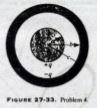
\includegraphics[scale=.7]{fig2733.jpg}
		\end{center}
		
	\end{problem}
	
	\begin{solution}
		\vfill
	\end{solution}
	\newpage

	\begin{problem}[HRK P27.5] 
A very long conducting cylinder (length $L$) carrying a total charge $+q$ is surrounded by a conducting cylindrical shell (also of length $L$) with total charge $-2q$, as shown in cross section in Fig. 27-34. Use Gauss's law to find (a) the electric field at points outside the conducting shell, (b) the distribution of the charge on the conducting shell, and (c) the electric field in the region between the cylinders.	
	\begin{center}
			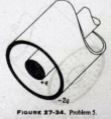
\includegraphics[scale=.7]{fig2734.jpg}
	\end{center}
	\end{problem}
	\begin{solution}
		\vfill
	\end{solution}
	\newpage

	\begin{problem}[HRK E27.29]
A metal plate 8.0 cm on a side carries a total charge of 6.0 $\mu$C. (a) Using the infinite plate approximation, calculate the electric field .50 mm above the surface of the plate near the plate's center. (b) Estimate the field at a distance of 30 m.
(Make sure to given an analytical answer before calculating a numerical answer with units.)
		
	\end{problem}
	
	\begin{solution}
		\vfill
	\end{solution}
	\newpage	
	
	\begin{problem}Consider an infinite, non-conducting, charged sheet of thickness $w$. Find the electric field inside and outside the sheet (amplitude and direction) if the volume charge density inside the sheet is $\rho = \frac{\rho_0|z|}{w}$, where z-axis is perpendicular to the plane of the sheet and z = 0 on the mid-plane
of the sheet.
	\end{problem}
	
	\begin{solution}
		\vfill
	\end{solution}
	\newpage
	
	\begin{problem}[Schey: II-26]
a) Use the divergence theorem to show that $\frac{1}{3} \varoiint_S \hat{\mathbf{n}} \cdot \vec{r} dA = V$ where $S$ is a closed surface enclosing a region of volume $V$, $\hat{\mathbf{n}}$ is a unit vector normal to the surface $S$, and $\vec{r} = x\hat{\mathbf{x}} + y\hat{\mathbf{y}} + z\hat{\mathbf{z}}$.\\
b) Use the result in (a) to find the volume of \\
i) a rectangular parallelepiped with sides $a, b, c$ \\
ii) a right circular cone with height $h$ and base radius $R$. [Hint: The calculation is very simple
with the cone oriented as shown in the figure on page 61 of Schey] \\
iii) a sphere of radius $R$.

		
	\end{problem}
	
	\begin{solution}
		\vfill
	\end{solution}
	\newpage
	
	\begin{problem}[(based on Schey II-14 and II-15]
a) For the vector function $\vec{F}(x,y,z) = e^{-x}\hat{\mathbf{x}} + e^{-y}\hat{\mathbf{y}} + e^{-z}\hat{\mathbf{z}}$.\\
i) Calculate the divergence of $\vec{F}$ and evaluate it at a point $(x_0, y_0, z_0$). \\
ii) Calculate $\varoiint_S \vec{F}\cdot \hat{\mathbf{n}} dA$ over the surface of a cube of side $a$ centered at the same point and whose  faces are parallel to the coordinate planes. \\
iii)  Divide the above result by the volume of the cube and calculate the limit of the quotient as
$a \rightarrow 0$. Compare your result with the divergence you calculated in part (i) and comment on your findings. \\
b) Now repeat the procedure in part (a) for the vector function $\vec{G}(x,y,z) = yz\hat{\mathbf{x}} + xz\hat{\mathbf{y}} + xt\hat{\mathbf{z}}$.
	\end{problem}
	
	\begin{solution}
		\vfill
	\end{solution}
	\newpage
	
	
\end{document}